\documentclass[11pt, A4paper,norsk]{article}
\usepackage[utf8]{inputenc}
\usepackage[T1]{fontenc}
\usepackage{babel}
\usepackage{amsmath}
\usepackage{amsfonts}
\usepackage{amsthm}
\usepackage[colorlinks]{hyperref}
\usepackage{listings}
\usepackage{color}
\usepackage{hyperref}
\usepackage{graphicx}
\usepackage{cite}

\definecolor{dkgreen}{rgb}{0,0.6,0}
\definecolor{gray}{rgb}{0.5,0.5,0.5}
\definecolor{daynineyellow}{rgb}{1.0,0.655,0.102}
\definecolor{url}{rgb}{0.1,0.1,0.4}

\lstset{frame=tb,
	language=Python,
	aboveskip=3mm,
	belowskip=3mm,
	showstringspaces=false,
	columns=flexible,
	basicstyle={\small\ttfamily},
	numbers=none,
	numberstyle=\tiny\color{gray},
	keywordstyle=\color{blue},
	commentstyle=\color{daynineyellow},
	stringstyle=\color{dkgreen},
	breaklines=true,
	breakatwhitespace=true,
	tabsize=3
}

\lstset{inputpath="C:/Users/Torstein/Documents/UiO/Mek1100/Python programmer"}
\hypersetup{colorlinks, urlcolor=url}

\author{Torstein Solheim Ølberg}
\title{Svar på Oblig nr.1 i Mek1100}

\begin{document}
\maketitle
	\begin{center}
\Large \textbf{Oppgaver}
	\end{center}









		\paragraph{1)}
En ball kastes ut fra origo over en flat horisontal bakke. x-aksen er horisontal langs
bakken og y-aksen peker vertikalt oppover. Ballen kastes ut med fart $v_0$ ved tiden
$t = 0$. Kastet kan innstilles med utkastvinkel $\theta$ i forhold til den horisontale $x$-aksen. Ballen vil følge en bane gitt ved
			\begin{align}
x(t) = v_0 t cos\theta \\
y(t) = v_0 t sin\theta - \frac{1}{2} g t^2
			\end{align}










			\subparagraph{a)}
				\begin{flushleft}
Finn tiden $t_m$ når ballen faller ned på bakken $(y = 0)$ og posisjonen $x(t_m) = x_m$
hvor dette skjer. \\
\vspace{1mm}
\textbf{Løsning:}
\vspace{1mm}
					\begin{align}
x(t) = v_0 t cos\theta \nonumber \\
y(t) = v_0 t sin\theta - \frac{1}{2} g t^2 \nonumber \\
\text{Skal finne tiden når $y = 0$ så setter $y(t) = 0$} \nonumber \\
\text{Derretter regner ut tiden dette er tilfellet.} \nonumber \\
0 = -2 \frac{v_0 t_m sin\theta}{g} + t_m^2 \nonumber \\
\text{Vi ser over at $t_m = 0$ gir en løsning.} \nonumber \\
\text{Den andre finner vi enkelt ved å dele alle leddene på $t_m$} \nonumber \\
0 = -2 \frac{v_0 sin\theta}{g} + t_m \nonumber \\
t_m = 2 \frac{v_0 sin\theta}{g} \nonumber \\
\text{Setter $t_m$ fra likningen over inn i likningen for $x(t)$} \nonumber \\
x_m = v_0 \frac{2 v_0 sin\theta}{g} cos\theta \Rightarrow x_m = \frac{2 v_0^2 sin\theta cos\theta}{g} \nonumber
					\end{align}
				\end{flushleft}









			\subparagraph{b)}
				\begin{flushleft}
Innfør dimensjonsløse variable $(x*, y* , t*)$ for $x, y, t$ når du skalerer med $x_m$ for lengde og $t_m$ for tid. Forklar hvorfor det ikke er behov for å skalere vinkelen $\theta$. \\
\vspace{1mm}
\textbf{Løsning:} \\
\vspace{1mm}
					\begin{align}
x* = \frac{x}{x_m} \nonumber \\
t* = \frac{t}{t_m} \nonumber \\
x = v_0 t cos\theta \nonumber \\
x* \frac{2 v_0^2 sin\theta cos\theta}{g} = t* \frac{2 v_0^2 sin\theta cos\theta}{g} \nonumber \\
x* = t* \nonumber \\
y* = \frac{y}{x_m} \nonumber\\
y = v_0 t sin\theta - \frac{1}{2} g t^2 \nonumber \\
y* \frac{2 v_0^2 sin\theta cos\theta}{g} = \frac{t* 2 v_0^2 sin^2\theta}{g} - \frac{g 4 v_0^2 sin^2\theta t*^2}{2 g^2} \nonumber \\
y* = \frac{sin\theta}{cos\theta} t* - \frac{sin\theta}{cos\theta}t*^2 = tan\theta t* - tan \theta t*^2 \nonumber
					\end{align}
				\end{flushleft}









			\subparagraph{c)}
				\begin{flushleft}
Bruk Matlab eller Python for å tegne baner $(x*, y*)$ for tre utkastvinkler $\theta_n$ for $n = 1, 2, 3$. Velg $0 < \theta_1 < \frac{\pi}{4}, \theta_2 = \frac{\pi}{4} og \frac{\pi}{4} < \theta_3 < \frac{\pi}{2}$. Tegn de tre banene i samme koordinatsystem, og angi hvilken bane som svarer til hvilken utkastvinkel. Forklar hvorfor disse diagrammene kan brukes til å finne ballens baner for forskjellige verdier av utgangsfart $v_0$ og forskjellige verdier av $g$. \\
\vspace{1mm}
\textbf{Løsning:} \\
\vspace{1mm}
				\end{flushleft}
\lstinputlisting{Oblig1_1c.py}
\includegraphics[width=12.6cm,height=8cm]{"C:/Users/Torstein/Documents/UiO/Mek1100/Python programmer"/Oblig1_1c.png}









		\paragraph{2)}
			\begin{flushleft}
Vi skal nå se på hastighetsfeltet $$\vec{v} = v_x\vec{i} + v_y\vec{j} = xy\vec{i} + y\vec{j}$$ \\
			\end{flushleft}
			\subparagraph{a}
				\begin{flushleft}
Finn strømlinjene.
HINT $1$: Du må løse ei differensiallikning som viser seg å være separabel, det vil si at den kan skrives om på formen $f(x)dx = g(y)dy$. \\
HINT $2$: Fanger du opp at $x$-aksen også er løsning av den opprinnelige differensiallikninga? \\
\vspace{1mm}
\textbf{Løsning:} \\
\vspace{1mm}
Du finner likningen for strømlinjene ved å ta $\vec{v} X d\vec{r}$.
					\begin{align}
\vec{v} X d\vec{r} =
\left|
\begin{tabular} {c c c}
i & j & k  \\
v_x & v_y & v_z  \\
dx & dy & dz  
\end{tabular}
\right| \nonumber
\textsl{}					\end{align}
			\end{flushleft}









		\subparagraph{b)}
			\begin{flushleft}
Tegn strømlinjene for hånd og sett på piler for å indikere retningen på strømmen. Et stagnasjonspunkt er et punkt hvor hastighetsfeltet er lik null. Finn alle stagnasjonspunktene og identifiser hvor i plottet disse ligger. Det er vanlig å tegne individuelle stagnasjonspunkter som tjukke kulepunkter $\bullet$. Vis også at du får til å tegne strømlinjene ved hjelp av Matlab eller Python, ved å bruke kommandoen contour. Dette kan kanskje vise seg å være en utfordring nær $x = 0$.
\\
\vspace{1mm}
\textbf{Løsning:} \\
\vspace{1mm}
\includegraphics[width=12.6cm,height=8cm]{"C:/Users/Torstein/Documents/UiO/Mek1100"/Oblig1_2b.png}
\lstinputlisting{oblig1_2b.py}
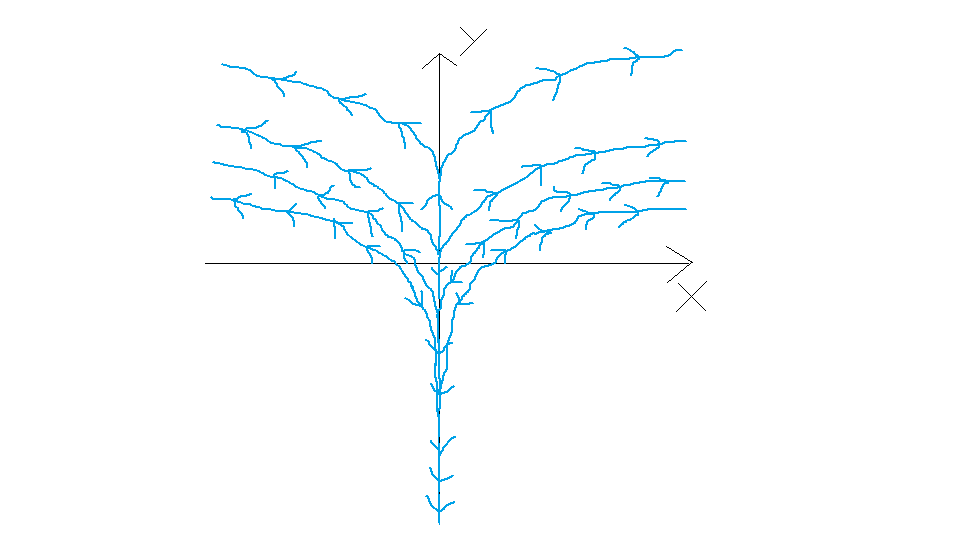
\includegraphics[width=12.6cm,height=8cm]{"C:/Users/Torstein/Documents/UiO/Mek1100/Python programmer"/oblig1_2b.png}
			\end{flushleft}









			\subparagraph{c)}
				\begin{flushleft}
Vis at det ikke finnes en strømfunksjon $\psi$. \\
HINT: En strømfunksjon $\psi(x, y)$ for et todimensjonalt felt $\vec{v} = v_x\vec{i} + v_y \vec{j}$ i $xy$-planet har egenskapen $v_x = -\dfrac{\partial \psi}{\partial y}$ og $vy = \dfrac{\partial \psi}{\partial x}$. Dersom en slik strømfunksjon eksisterer så er strømlinjene gitt ved ekviskalarkurvene til strømfunksjonen, $\psi(x, y) =$ konstant.
Dersom et vektorfelt er todimensjonalt i $xy$-planet, $\vec{v} = v_x\vec{i} + v_y\vec{j}$ og divergensfritt, $\dfrac{\partial v_x}{\partial x} + \dfrac{\partial v_y}{\partial y} = 0$, så eksisterer det en strømfunksjon som angitt ovenfor. Dersom et vektorfelt har divergens forskjellig fra null, så eksisterer det ikke en strømfunksjon for feltet. For å vise at et felt ikke har en strømfunksjon, kan man enten vise at forsøk på å regne den ut ender i en selvimotsigelse, eller man kan vise at divergensen til feltet er ulik null. \\
\vspace{1mm}
\textbf{Løsning:} \\
\vspace{1mm}
Viser at divergensen til feltet ikke er lik null $$\nabla \cdot \vec{v} = \frac{\partial v_x}{\partial x} + \frac{\partial v_y}{\partial x} = y + 1 $$ Dette er ikke lik $0$, som vil si at det ikke finnes noen strømfunksjon for feltet.
			\end{flushleft}









		\paragraph{3)}
			\begin{flushleft}
Et hastighetsfelt i $xy$-planet er gitt ved $\vec{v} = v_x\vec{i} + v_y\vec{j}$ der
$$v_x = cos(x) sin(y), v_y = - sin(x) cos(y)$$
			\end{flushleft}
			\subparagraph{a)}
				\begin{flushleft}
Finn divergensen $\nabla \cdot \vec{v} = \frac{\partial v_x}{\partial x} + \frac{\partial v_y}{\partial y}$ og virvlingen $\nabla X \vec{v} = (\frac{\partial v_y}{\partial x} - \frac{\partial v_x}{\partial y}) \vec{k}$ av hastighetsfeltet. \\
\vspace{1mm}
\textbf{Løsning:} \\
\vspace{1mm}
					\begin{align}
\nabla \cdot \vec{v} = \dfrac{\partial v_x}{\partial x} + \dfrac{\partial v_y}{\partial y} = -sin(x)sin(y) + sin(x)sin(y) = 0 \nonumber \\
\nabla X \vec{v} = (\frac{\partial v_y}{\partial x} - \frac{\partial v_x}{\partial y}) \vec{k} = -cos(x)cos(y) - cos(x)cos(y)\vec{k} \nonumber \\
\nabla X \vec{v} = -2cos(x)cos(y) \vec{k} \nonumber
					\end{align}
				\end{flushleft}












			\subparagraph{b)}
				\begin{flushleft}
Tegn opp strømvektorer langs $x$- og $y$-aksen. \\
\vspace{1mm}
\textbf{Løsning:} \\
\vspace{1mm}
Plottet med quiverfunksjonen i python.
\lstinputlisting{oblig1_3b.py}
\includegraphics[width=12.6cm,height=8cm]{"C:/Users/Torstein/Documents/UiO/Mek1100/Python programmer"/Oblig1_3b.png}
				\end{flushleft}












			\subparagraph{c)}
				\begin{flushleft}
Finn sirkulasjonen om randa til kvadratet definert ved $- \frac{\pi}{2} \geq x \leq  \frac{\pi}{2}$ og $- \frac{\pi}{2} \geq y \leq \frac{\pi}{2}$. \\
\vspace{1mm}
\textbf{Løsning:} \\
\vspace{1mm}
					\begin{align}
\Delta C = \oint \vec{v} \cdot d \vec{r} = \int_{a}^{b} \vec{v} \cdot d\vec{r} + \int_{b}^{c} \vec{v} \cdot d\vec{r} + \int_{c}^{d} \vec{v} \cdot d\vec{r} + \int_{d}^{a} \vec{v} \cdot d\vec{r} \nonumber \\
\int_{a}^{b} \vec{v} \cdot d\vec{r} = \int_{- \frac{\delta x}{2}}^{\frac{\delta x}{2}} v_x(x, -\frac{\delta y}{2}) dx = \int_{-\frac{\pi}{2}}^{\frac{\pi}{2}} cos(x)sin(- \frac{\pi}{2}) dx \nonumber \\
\int_{a}^{b} \vec{v} \cdot d\vec{r} = \left[-sin(x)sin(-\frac{\pi}{2})\right]_{-\frac{\pi}{2}}^{\frac{\pi}{2}} = sin(\frac{\pi}{2})sin(\frac{\pi}{2}) - sin(- \frac{\pi}{2})sin(- \frac{\pi}{2}) \nonumber \\
\Delta C = -2 \nonumber \\
\int_{b}^{c} \vec{v} \cdot d\vec{r} = \int_{-\frac{\delta y}{2}}^{\frac{\delta y}{2}} v_y(\frac{\delta x}{2}, y) dy = \int_{\frac{\pi}{2}}^{\frac{\pi}{2}} -sin(\frac{\pi}{2})cos(y) dy \nonumber \\
\int_{b}^{c} \vec{v} \cdot d\vec{r} = \left[sin(\frac{\pi}{2})sin(y)\right]_{-\frac{\pi}{2}}^{\frac{\pi}{2}} = sin(\frac{\pi}{2})sin(\frac{\pi}{2}) - sin(-\frac{\pi}{2})sin(-\frac{\pi}{2}) \nonumber \\
 = -2 \nonumber \\
\int_{c}^{d} \vec{v} \cdot d\vec{r} = \int_{\frac{\delta x}{2}}^{-\frac{\delta x}{2}} v_x(x, \frac{\delta y}{2}) dx = \int_{\frac{\pi}{2}}^{-\frac{\pi}{2}} cos(x)sin(\frac{\pi}{2}) dx \nonumber \\
\int_{c}^{d} \vec{v} \cdot d\vec{r} = \left[-sin(x)sin(\frac{\pi}{2})\right]_{\frac{\pi}{2}}^{-\frac{\pi}{2}} = sin(-\frac{\pi}{2})sin(\frac{\pi}{2}) - sin(-\frac{\pi}{2})sin(\frac{\pi}{2}) \nonumber \\
\Delta C = -2 \nonumber \\
\int_{d}^{a} \vec{v} \cdot d\vec{r} = \int_{\frac{\delta y}{2}}^{-\frac{\delta y}{2}} v_y(-\frac{\delta x}{2}, y) dy = \int_{\frac{\pi}{2}}^{- \frac{\pi}{2}} -sin(-\frac{\pi}{2})cos(y) dy \nonumber \\
\int_{d}^{a} \vec{v} \cdot d\vec{r} = \left[sin(-\frac{\pi}{2})sin(y)\right]_{\frac{\pi}{2}}^{-\frac{\pi}{2}} = sin(-\frac{\pi}{2})sin(\frac{\pi}{2}) - sin(-\frac{\pi}{2})sin(-\frac{\pi}{2}) \nonumber \\
\Delta C = -2 \nonumber \\
\Delta C = -2-2-2-2 = -8 \nonumber 
					\end{align}
				\end{flushleft}









			\subparagraph{d)}
				\begin{flushleft}
Forklar hvorfor det eksisterer en strømfunksjon for feltet gitt i likning (1), se hintet gitt i forrige oppgave. Vis at strømfunksjonen kan skrives $psi = cos(x) cos(y)$. \\
\vspace{1mm}
\textbf{Løsning:} \\
\vspace{1mm}
Hvis $\nabla \cdot \vec{v} = 0$, noe vi viste i oppgave a, så må det finnes en $\psi$ som er strømfunksjonen til vektorfeltet $\vec{v}$.
					\begin{align}
\psi = - \int v_x dy \vee \psi = \int v_y dx\nonumber \\
\psi = - \int cos(x)sin(y)dy = -\left[-cos(x)cos(y)\right] \nonumber \\
\psi = \int -sin(x)cos(y) = \left[cos(x)cos(y)\right] \nonumber \\
\text{Ser av de to likningene over at}
\psi = cos(x)cos(y)
					\end{align}
				\end{flushleft}










			\subparagraph{e)}
				\begin{flushleft}
Bruk Taylorutvikling av andre orden til å finne tilnærmede strømlinjer nær origo. \\
\vspace{1mm}
\textbf{Løsning:} \\
\vspace{1mm}
					\begin{align}
\psi = cos(x)cos(y) \nonumber \\
\frac{\partial \psi}{\partial x} = -sin(x)cos(y) \nonumber \\
\frac{\partial \psi}{\partial y} = -cos(x)sin(y) \nonumber \\
\frac{\partial^2 \psi}{\partial^2 x} = -cos(x)cos(y) \nonumber \\
\frac{\partial^2 \psi}{\partial x \partial y} = sin(x)sin(y) \nonumber \\
\frac{\partial^2 \psi}{\partial y \partial x} = -sin(x)sin(y) \nonumber \\
\frac{\partial^2 \psi}{\partial^2 y} = -cos(x)cos(y) \nonumber \\
T_2 \psi = 1 -0 -0 -\frac{x^2}{2!} -\frac{y^2}{2!} \nonumber
					\end{align}
				\end{flushleft}
\lstinputlisting{oblig1_3e.py}
\includegraphics[width=12.6cm,height=8cm]{"C:/Users/Torstein/Documents/UiO/Mek1100/Python programmer"/Oblig1_3e.png}








		\paragraph{4)}
			\begin{flushleft}
I denne oppgaven skal du skrive noen funskjoner og skript i Matlab eller Python. Disse og de plott som produseres skal leveres inn som en del av besvarelsen. Det er viktig at de filene du lager har de navn som oppgis. Alle figurer skal ha tittel og tekst på akser.
Sammen med oppgaveteksten, på hjemmesiden, finner du filene streamfun.m og streamfun.py med en funksjon som beregner strømfunksjonen (2) i området. Et kall på funksjonen kan i Matlab se ut som $$\gg [x,y,psi]=streamfun(n);$$ og kan i Python se ut som $$\gg x,y,psi=streamfun(n)$$ der x,y,psi er arrayer for henholdsvis $x$-verdier, $y$-verdier og $\psi$. Inngangsparameteren $n$ er antall punkter som brukes i hver retning. Avstanden mellom punktene, i begge retninger, blir da $\delta x = \delta y = \frac{\pi}{n - 1}$.
			\end{flushleft}












			\subparagraph{a)}
				\begin{flushleft}
Bruk funksjonen streamfun i et skript, strlin.m eller strlin.py, som plotter konturlinjer for $\psi$ når
					\begin{align}
(i) n = 5 \nonumber \\
(ii) n = 30 \nonumber
					\end{align}
Framstill tilfellene (i) og (ii) i hvert sitt diagram. Sammenhold plottene med punkt e) i forrige oppgave og diskuter de valgte verdier for $n$. \\
\vspace{1mm}
\textbf{Løsning:} \\
\vspace{1mm}
\lstinputlisting{strlin.py}
\includegraphics[width=12.6cm,height=8cm]{"C:/Users/Torstein/Documents/UiO/Mek1100/Python programmer"/strlin1.png}
\includegraphics[width=12.6cm,height=8cm]{"C:/Users/Torstein/Documents/UiO/Mek1100/Python programmer"/strlin2.png}
Som vi ser av plottene så er en større n-verdi lurt fordi det gir en glattere og sannsynligvis mer nøyaktig kurve. Når vi sammenlikner med oppgave 3e) ser vi at vi får de samme strømlinjene, noe som gir mening siden vi bruker samme strømlinjefunksjon.
			\end{flushleft}









			\subparagraph{b)}
				\begin{flushleft}
Skriv en funksjon (filnavn velfield.m eller velfield.py) som beregner hastigheter utfra likning (1) ved kallet $$\gg [x,y,u,v]=velfield(n);$$ eller $$\gg x,y,u,v=velfield(n)$$ Bruk denne i et skript, vec.m eller vec.py, som tegner et vektorplott av hastighetsfeltet. Legg vekt på å velge et passende antall punkter for lesbarheten av plottet. \\
\vspace{1mm}
\textbf{Løsning:} \\
\vspace{1mm}
\lstinputlisting{velfield.py}
\lstinputlisting{vec.py}
\includegraphics[width=12.6cm,height=8cm]{"C:/Users/Torstein/Documents/UiO/Mek1100/Python programmer"/vec.png}
				\end{flushleft}
\end{document}